%!TEX options=--shell-escape
\documentclass[tikz]{standalone}
\usepackage[T1]{fontenc}
\usepackage[utf8]{inputenc}
\usepackage{xcolor}
\usepackage{amsmath}
\usepackage{amssymb}
\usepackage{hyperref}
\usepackage{accsupp}    
\usepackage{graphicx}
\usepackage{mathtools}
\usepackage{pagecolor}
\usepackage{amsmath} % for \dfrac
\usepackage{tikz,ifthen}
\tikzset{>=latex} % for LaTeX arrow head
\usepackage{braket}
\usepackage{pgfplots} 
\usepackage[edges]{forest}
\usetikzlibrary{patterns, backgrounds, arrows.meta}
\setlength{\parindent}{0cm}
\setlength{\parskip}{1em}

\usetikzlibrary{patterns, calc, intersections, shapes.geometric, fit}

\def\wheelwidth{1}
\def\wheelheight{1.5}

\def\axlelength{2}
\def\axelwidth{0.25}

\def\skateangle{5}

\def\platelength{3.5}
\def\platewidth{0.55}

\begin{document}

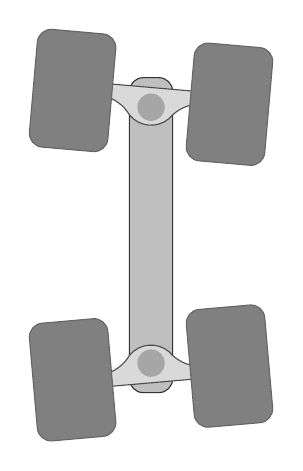
\begin{tikzpicture}[]


% Plate
\draw[black!80, fill=gray!50, rounded corners = 0.5em] (-0.5 * \platewidth, 0.5 * \platelength + \axelwidth) rectangle(0.5 * \platewidth, -0.5 * \platelength - \axelwidth);

% Front Axle
\draw[black!70, fill=gray!30, rotate around={-\skateangle:(0, 0.5 * \platelength)}] (0.5 * \axlelength, 0.5 * \platelength - 0.5 * \axelwidth) -- (0.5 * \axlelength, 0.5 * \platelength + 0.5 * \axelwidth) -- (-0.5 * \axlelength, 0.5 * \platelength + 0.5 * \axelwidth) -- (-0.5 * \axlelength, 0.5 * \platelength - 0.5 * \axelwidth) to [bend left=45] (-\axelwidth, 0.5 * \platelength - \axelwidth) to [bend right=45] (+\axelwidth, 0.5 * \platelength - \axelwidth) to [bend left=45] (0.5 * \axlelength, 0.5 * \platelength - 0.5 * \axelwidth);

\node[circle, black!70, inner sep = 0.35em, fill=gray!70] () at (0, \platelength * 0.5 - 0.5 * \axelwidth) {} ;

% Rear Axle
\draw[black!70, fill=gray!30, rotate around={\skateangle:(0, -0.5 * \platelength)} ] (0.5 * \axlelength, -0.5 * \platelength + 0.5 * \axelwidth) -- (0.5 * \axlelength, -0.5 * \platelength - 0.5 * \axelwidth) -- (-0.5 * \axlelength, -0.5 * \platelength - 0.5 * \axelwidth) -- (-0.5 * \axlelength, -0.5 * \platelength + 0.5 * \axelwidth) to [bend right=45] (-\axelwidth, -0.5 * \platelength + \axelwidth) to [bend left=45] (+\axelwidth, -0.5 * \platelength + \axelwidth) to [bend right=45] (0.5 * \axlelength, -0.5 * \platelength + 0.5 * \axelwidth);

\node[circle, black!70, inner sep = 0.35em, fill=gray!70] () at (0, \platelength * -0.5 + 0.5 * \axelwidth) {} ;





\draw[black!60, rounded corners=0.5em, fill=black!50, rotate around={-\skateangle:(0, 0.5 * \platelength)}] (0.5 * \axlelength + 0.5 * \wheelwidth, 0.5 * \platelength + 0.5 * \wheelheight) rectangle (0.5 * \axlelength - 0.5 * \wheelwidth, 0.5 * \platelength - 0.5 * \wheelheight) ; 

\draw[black!60, rounded corners=0.5em, fill=black!50, rotate around={-\skateangle:(0, 0.5 * \platelength)}] (-0.5 * \axlelength + 0.5 * \wheelwidth, 0.5 * \platelength + 0.5 * \wheelheight) rectangle (-0.5 * \axlelength - 0.5 * \wheelwidth, 0.5 * \platelength - 0.5 * \wheelheight) ; 


\draw[black!60, rounded corners=0.5em, fill=black!50, rotate around={\skateangle:(0, -0.5 * \platelength)}] (0.5 * \axlelength + 0.5 * \wheelwidth, -0.5 * \platelength + 0.5 * \wheelheight) rectangle (0.5 * \axlelength - 0.5 * \wheelwidth, -0.5 * \platelength - 0.5 * \wheelheight) ; 

\draw[black!60, rounded corners=0.5em, fill=black!50, rotate around={\skateangle:(0, -0.5 * \platelength)}] (-0.5 * \axlelength + 0.5 * \wheelwidth, -0.5 * \platelength + 0.5 * \wheelheight) rectangle (-0.5 * \axlelength - 0.5 * \wheelwidth, -0.5 * \platelength - 0.5 * \wheelheight) ; 


\end{tikzpicture} 



\end{document}

